% ===========================================================================
% OWNER: M2 (Abdul Raffay) for 5.1-5.5; M1 for 5.6-5.8 (in chapter5_data_behaviour.tex)
% GRADED BY: Form 3 #5 Architecture & component/interface design (15) - gate: diagrams must match the code
% DRAW FROM: docs/03-Design/architecture.md, docs/contracts/interfaces.md, report-schema.md, resource-evidence.md, docs/03-Design/decisions/ADR-001..008, runner/, evidence/, eval/ READMEs
% NOTE: Design Evolution must show the proposal block diagram next to the current architecture and say what changed and which ADR changed it
% Rules: mid-eval-report/CLAUDE.md. Do not edit a file you do not own.
% ===========================================================================
\chapter{System Design}
\section{System Architecture}
% Current architecture (M2): diagrams/m2/architecture.puml -> figures/m2/architecture.png
\placeholderfig{ch5:fig:arch}{FlakeTrace architecture at Iteration 1 (as implemented)}{M2}
\section{Architectural Components}
\section{Interfaces and Dependencies}
\section{Architecture Decisions and Rationale}
\section{Design Evolution}
Show important design changes since the proposal and justify them.
\begin{figure}[H]\centering
  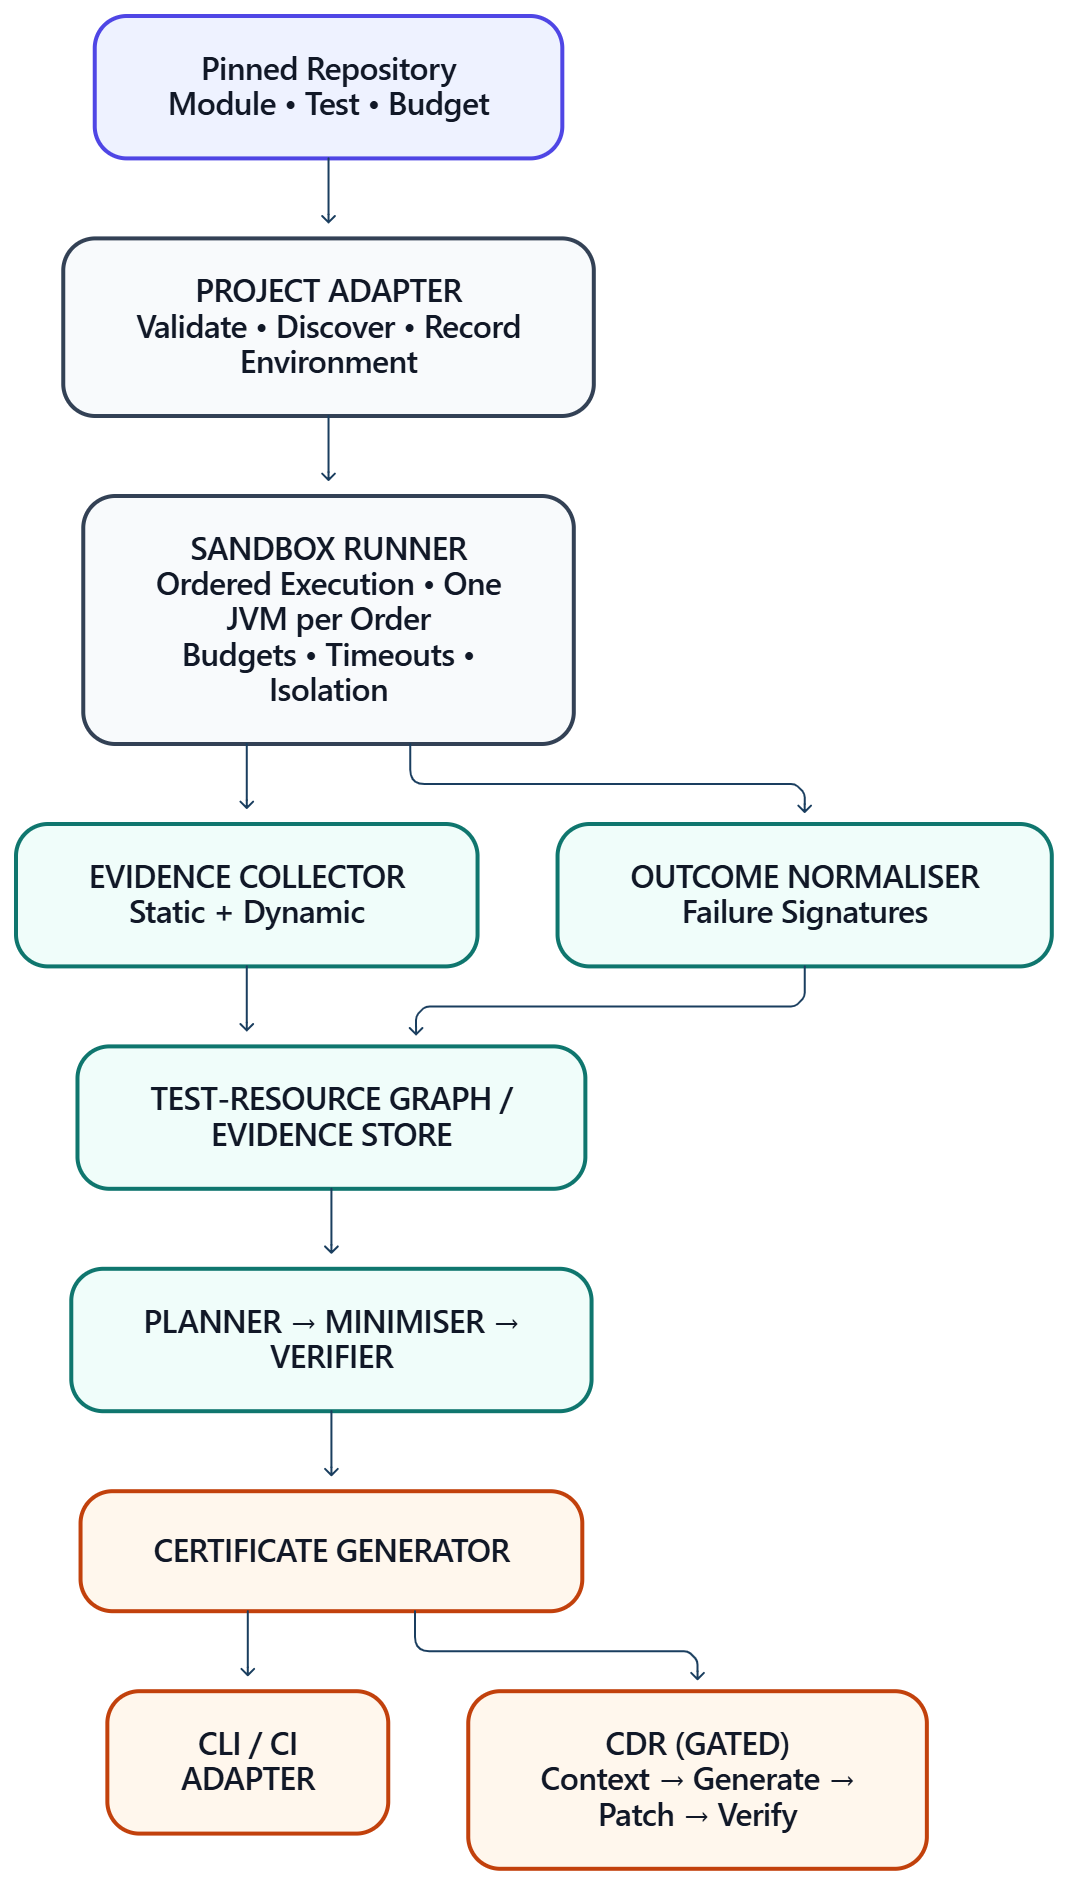
\includegraphics[width=0.85\textwidth]{figures/shared/proposal_block_diagram}
  \caption{System block diagram as presented at the proposal defence}\label{ch5:fig:proposal-arch}
\end{figure}
% Sections 5.6-5.8 are owned by M1:
% ===========================================================================
% OWNER: M1 (Zoya Ahmad); diagrams contributed by M2 and M3 as listed below
% GRADED BY: Form 3 #6 Data / process / behaviour design (10) - artefacts must be project-specific and explained in text
% DRAW FROM: eval/schema/report.schema.json, docs/contracts/*, evidence/extract.py, runner/diagnose.py, search.py, minimise.py, verify.py, eval/outcome.py
% NOTE: Each diagram is explained in prose: what it shows, and which code it was drawn from
% Rules: mid-eval-report/CLAUDE.md. Do not edit a file you do not own.
% ===========================================================================
% Included from chapter5_design.tex — no \chapter here.
\section{Domain Model}
\section{Data Design}
% Report data model (M1): diagrams/m1/report_data_model.puml -> figures/m1/report_data_model.png
\placeholderfig{ch5:fig:datamodel}{Diagnosis report data model (from report.schema.json)}{M1}
\section{Process / Behavior Design}
Include appropriate activity, sequence, state, DFD, ERD/schema, class, component, or other project-specific artefacts.
% Evidence extraction data flow (M1): diagrams/m1/evidence_dataflow.puml
\placeholderfig{ch5:fig:evidence-dfd}{Static evidence extraction: from bytecode to resource edges}{M1}
% Diagnose sequence (M2): diagrams/m2/diagnose_sequence.puml
\placeholderfig{ch5:fig:diagnose-seq}{Sequence of a \texttt{diagnose} run across the three components}{M2}
% Search pipeline activity (M2): diagrams/m2/search_activity.puml
\placeholderfig{ch5:fig:search-activity}{Reproduce, polluter search, minimisation and verification}{M2}
% Outcome decision (M3): diagrams/m3/outcome_decision.puml
\placeholderfig{ch5:fig:outcome}{Outcome decision: Verified, Candidate and typed Unresolved reasons}{M3}

